\section{Mise en place d'apache avec Kerberos}
\subsection{Objectifs et pré-requis}

Nous cherchons ici à mettre en place un système d'authentification sécurisée via Kerberos \footnote{Kerberos est un protocole réseau d'authentification. Il a été conçu pour apporter une authentification sûre pour un couple client/serveur en utilisant des clés de chiffrement. Il existe une implémentation gratuite de ce protocole par le MIT. Kerberos est aussi disponible dans plusieurs produits commerciaux - \url{https://web.mit.edu/kerberos/}}. \\
Pour cela, nous considérons que nous avons un serveur Windows 2012 déjà configuré via le présent document.

Ci-dessous, le comportement attendu de kerberos sur notre infrastructure :
\begin{figure}[h!]
     \begin{center}
         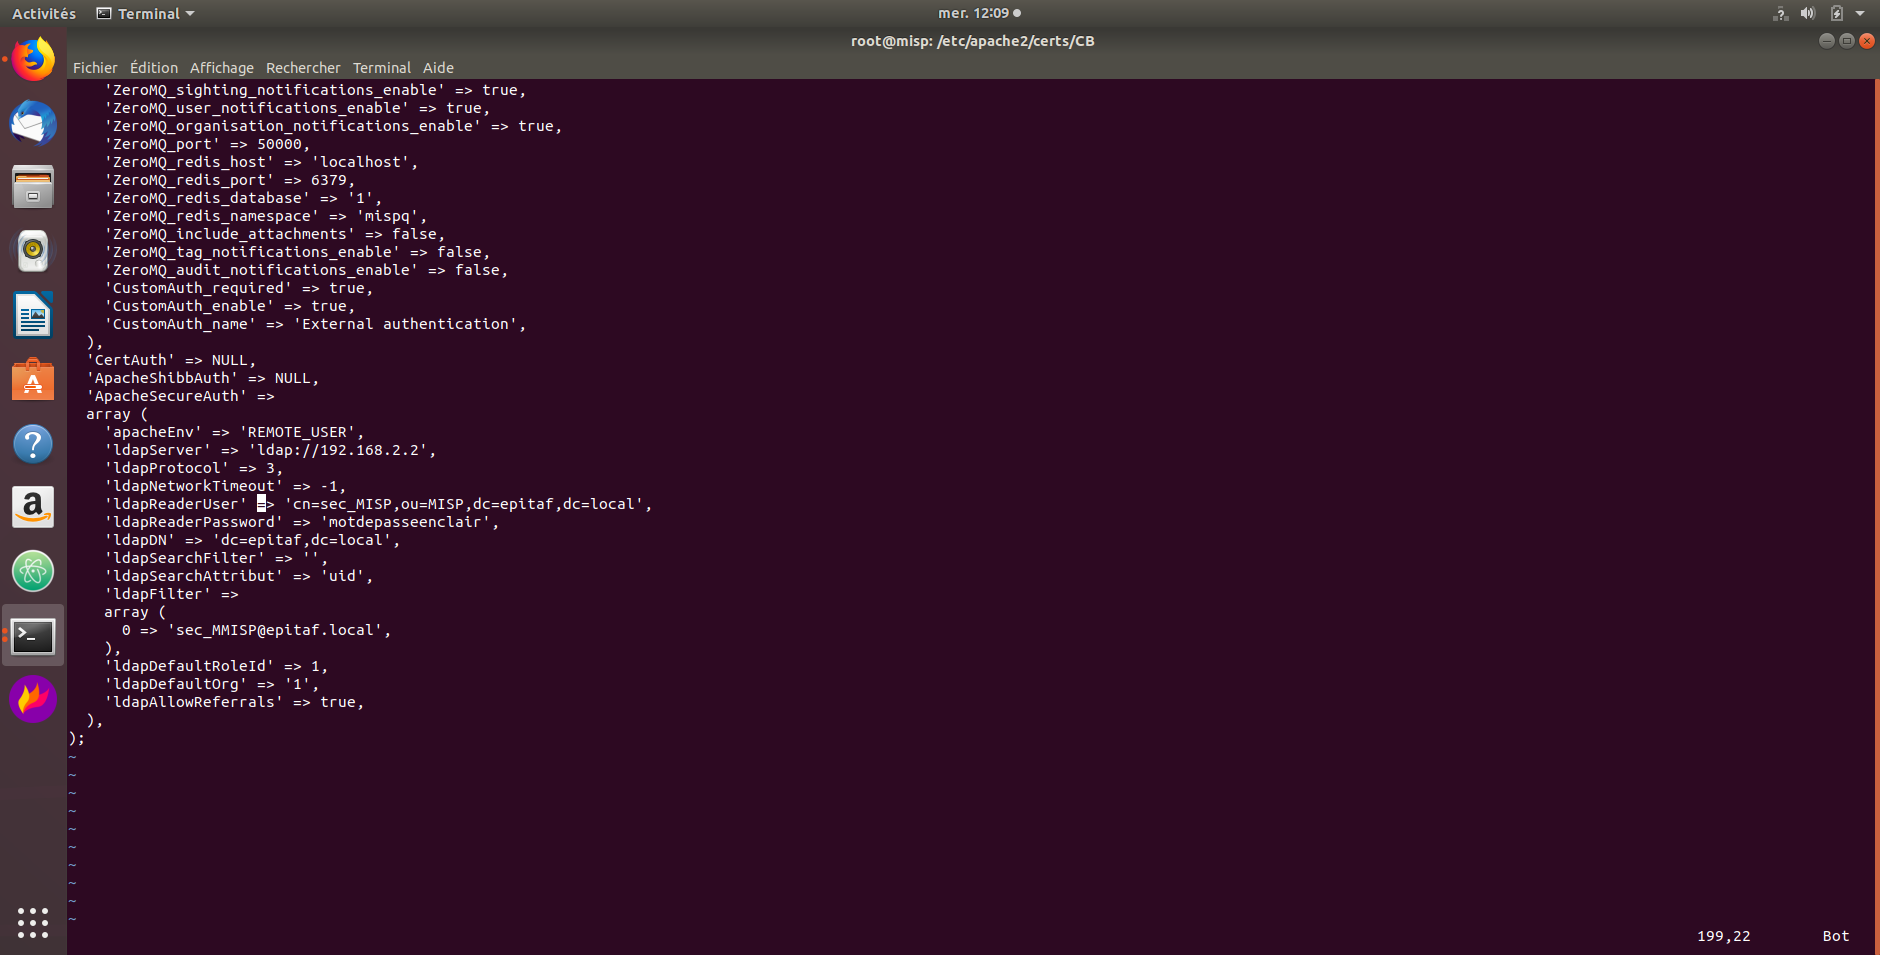
\includegraphics[scale=0.25]{Kerberos/kerberos.jpg}
         \caption{Schéma de la négociation avec le KDC}
         \label{Debian_screenshots/Config/5}
     \end{center}
  \end{figure}
  \FloatBarrier
  \newpage
  
 Il faut comprendre :
 \begin{itemize}
    \item \textbf{Mot de passe} : l'utilisateur du domaine \texttt{EPITAF} rentre son mot de passe ;
     \item \textbf{Hash} : le mot de passe est ensuite hashé par l'un des algorithmes et peut être retrouvé via LSSAS.exe;
     \item \textbf{AS-REQ} : la machine de l'utilisateur demande un ticket d'authentification au serveur windows qui est contrôleur de domaine et KDC;
     \item \textbf{AS-REP} : le KDC vérifie les identifiants et renvoie un ticket TGT et une clef de session chiffrés ;
     \item \textbf{TGS-REQ} : quand l'utilisateur cherchera à se connecter à un service, il enverra son ticket TGT et le nom du service auquel il veut accéder au Windows Server;
     \item \textbf{TGS-REP} : le KDC vérifie ensuite le TGT et l'accès au service auquel l'utilisateur veut accéder. Il renverra un ticket TGS permettant à l'utilisateur d'accéder au service voulu ;
     \item \textbf{TGS} : le client envoie son ticket TGS récemment reçu au serveur pour montrer qu'il peut accéder au service ;
     \item \textbf{Data} : le serveur fournit le service.
 \end{itemize}

\paragraph{}

  Afin de pouvoir mettre en place ce comportement, on devra : 
  \begin{itemize}
      \item Configurer le Windows Server (ktpass, création de services, etc) ;
      \item Configurer Apache pour qu'il puisse prendre en compte Kerberos ;
      \item Configurer les clients qui ne sont pas dans l'AD avec krb5-user ;
      \item Modifier la configuration des navigateurs internet pour qu'ils puissent prendre en compte la négociation kerberos.
  \end{itemize}
  
\pagebreak
  \subsection{Configuration de Windows Server}
  Dans \textit{Gestionnaire de serveur -> Outils}, cliquer sur DNS
  \begin{figure}[h!]
     \begin{center}
         
\includegraphics[scale=0.5]{Kerberos/1.png}
         \caption{Accès à la configuration DNS de Windows Server pour Kerberos}
         \label{Debian_screenshots/Config/5}
     \end{center}
  \end{figure}
  \FloatBarrier

\pagebreak
  Dans \textit{DNS -> DC01 -> Zones de recherche directes}, cliquer droit sur EPITAF.LOCAL puis cliquer sur \textbf{Nouvel hôte (A ou AAAA)...}
  \begin{figure}[h!]
     \begin{center}
         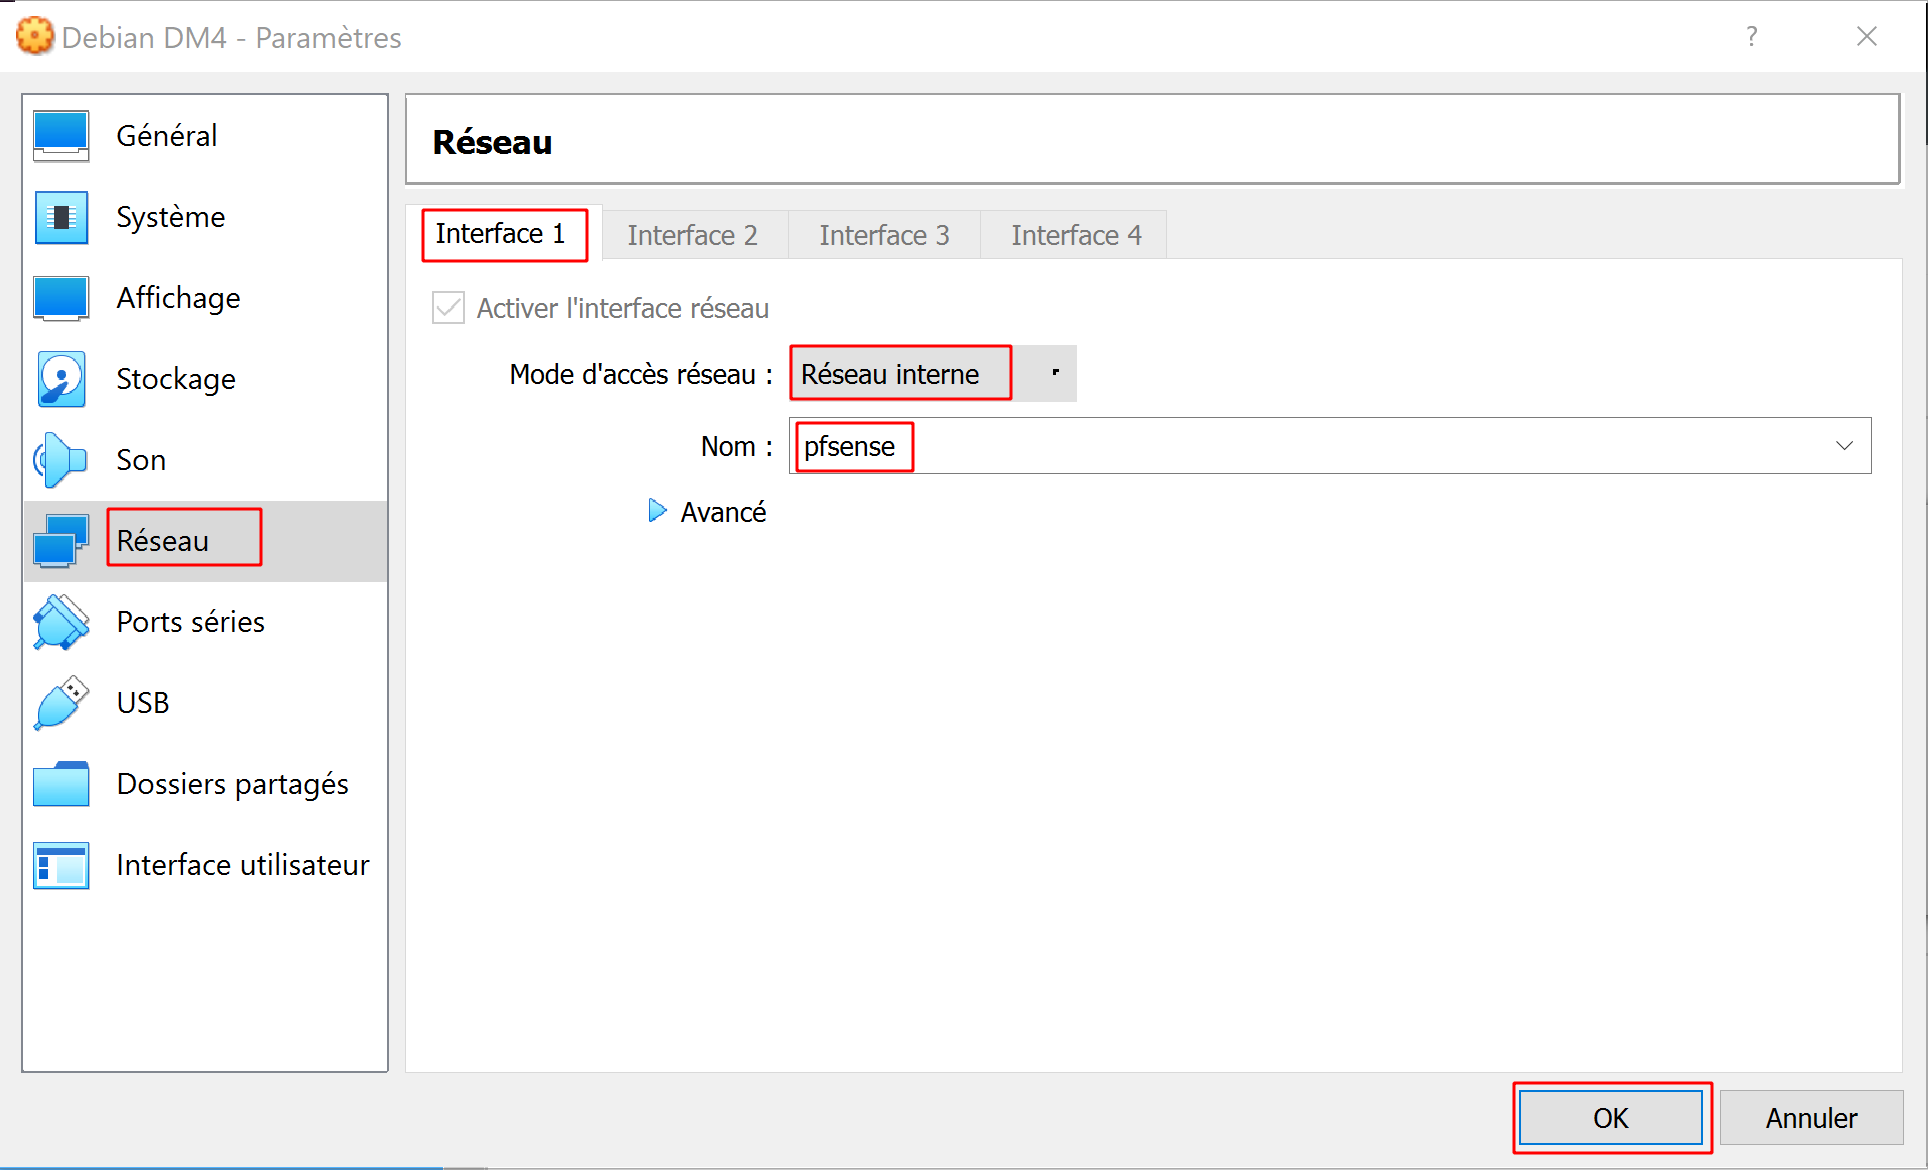
\includegraphics[scale=0.5]{Kerberos/2.png}
         \caption{Assertion d'une nouvelle entrée dans la DNS pour Kerberos}
         \label{Debian_screenshots/Config/5}
     \end{center}
  \end{figure}
  \FloatBarrier

\pagebreak
  Dans \textbf{Nom} mettre \textit{infra01} ; dans \textbf{Adresse IP} mettre \textit{192.168.3.2} ; cliquer sur \textbf{Ajouter un hôte}
  \begin{figure}[h!]
     \begin{center}
         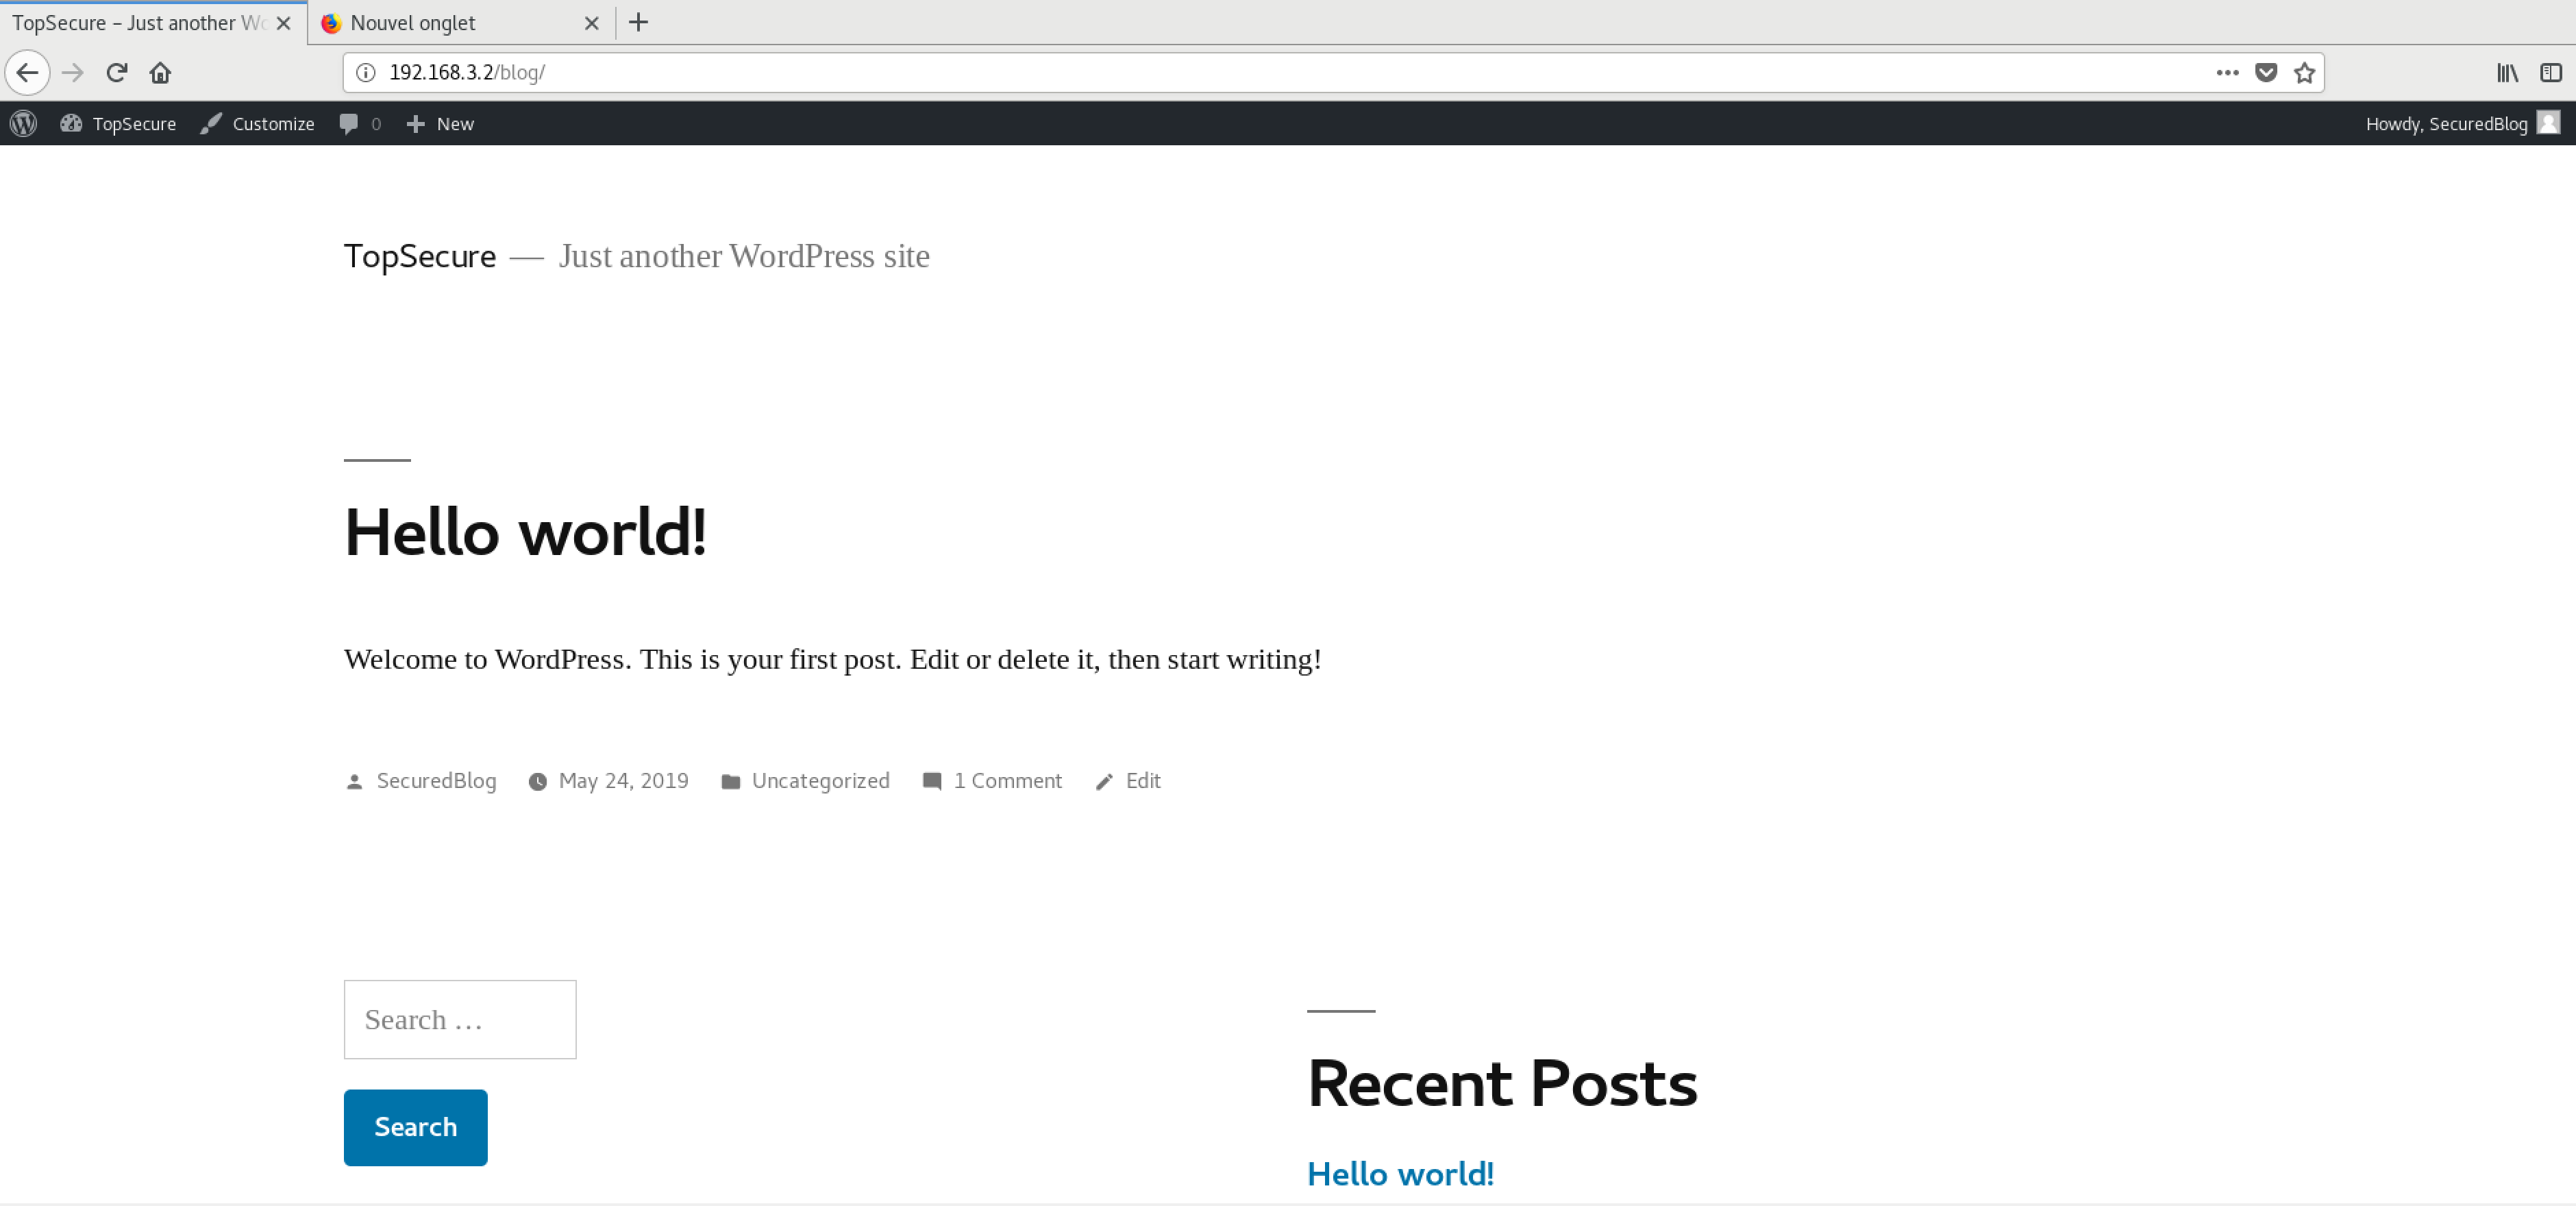
\includegraphics[scale=0.5]{Kerberos/3.png}
         \caption{Ajout d'un nouvel hôte pour Kerberos}
         \label{Debian_screenshots/Config/5}
     \end{center}
  \end{figure}
  \FloatBarrier

\pagebreak
  Dans \textit{Gestionnaire de serveur -> Outils}, cliquer sur \textbf{Centre d'administration Active Directory}
  \begin{figure}[h!]
     \begin{center}
         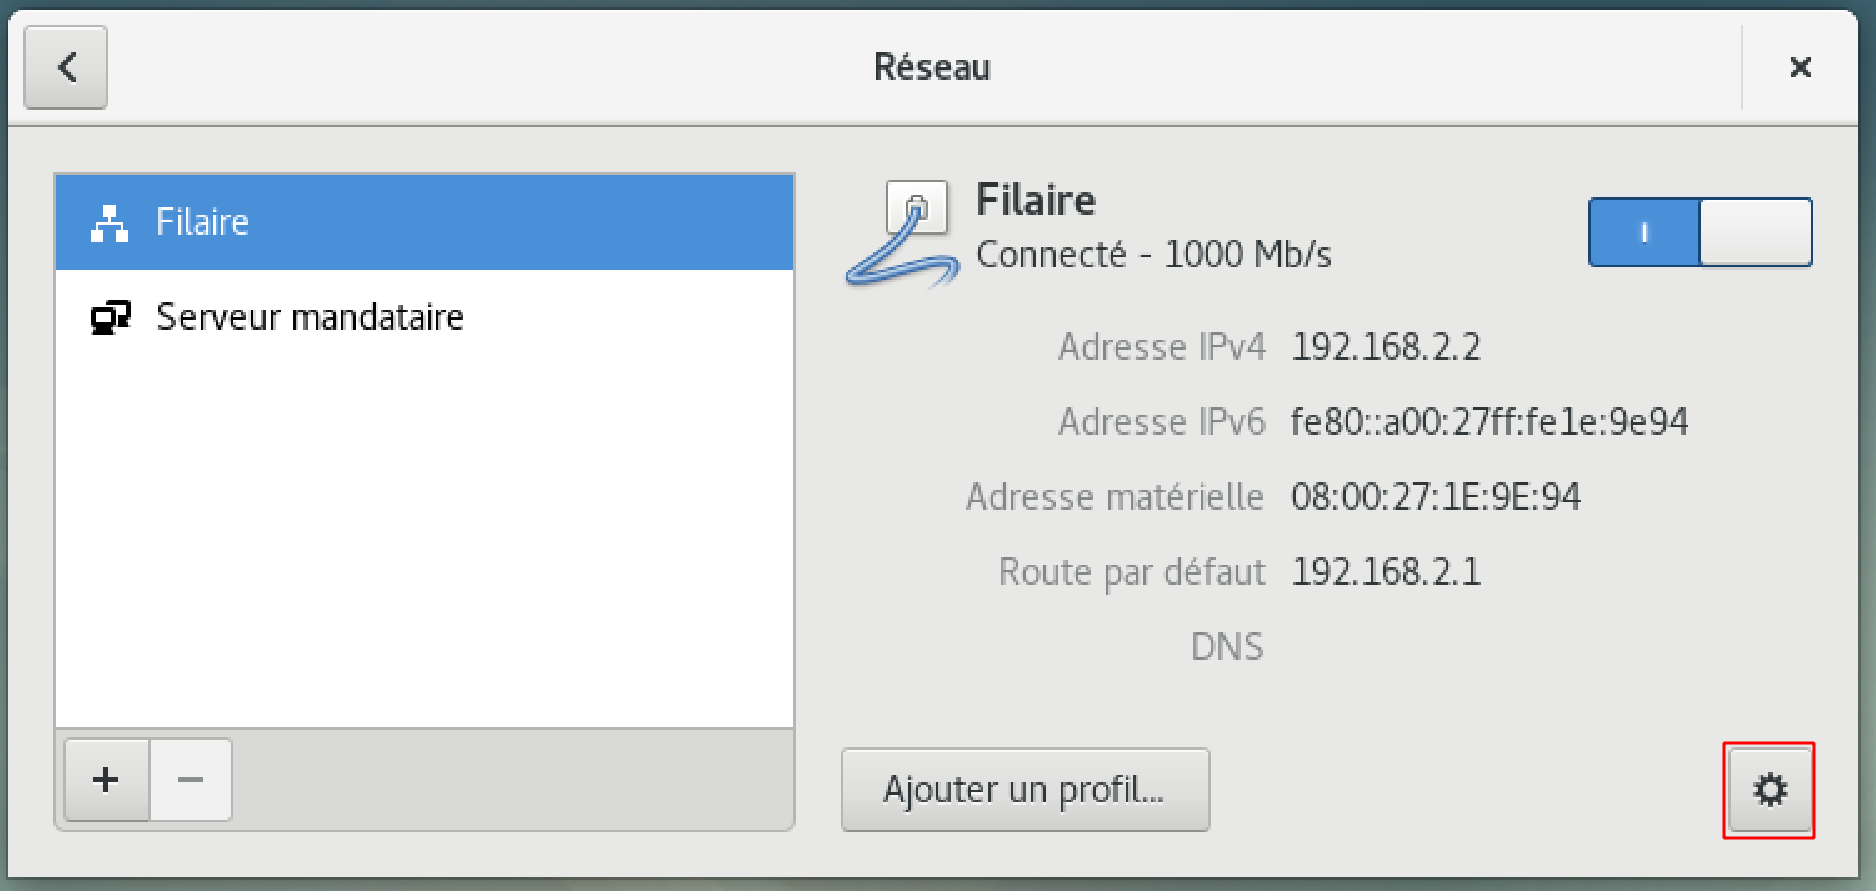
\includegraphics[scale=0.5]{Kerberos/4.png}
         \caption{Accès au centre d'administration Active Directory}
         \label{Debian_screenshots/Config/5}
     \end{center}
  \end{figure}
  \FloatBarrier

\pagebreak
   Dans le centre d'administration Active Directory, cliquer droit sur EPITAF (local) puis dans \textit{Nouveau}, cliquer sur \textbf{Utilisateur}
  \begin{figure}[h!]
     \begin{center}
         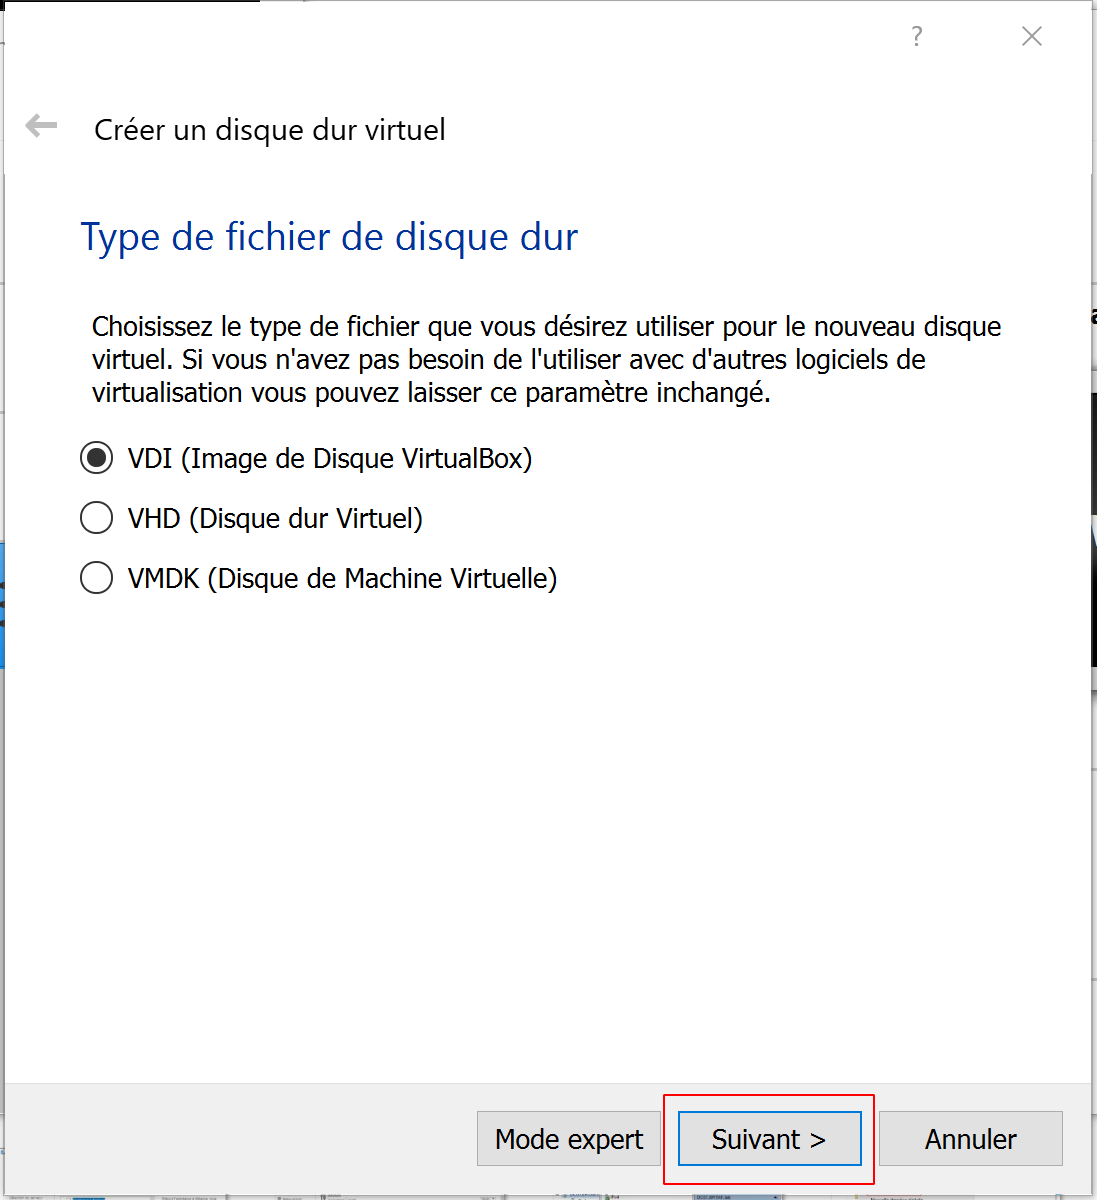
\includegraphics[scale=0.5]{Kerberos/5.png}
         \caption{Création d'un nouvel utilisateur}
         \label{Debian_screenshots/Config/5}
     \end{center}
  \end{figure}
  \FloatBarrier

\pagebreak
    Dans \textbf{Prénom} mettre \textit{apache} ; dans \textbf{Ouverture de session} mettre \textit{apache} ; entrer un mot de passe puis cliquer sur \textbf{Ok}
  \begin{figure}[h!]
     \begin{center}
         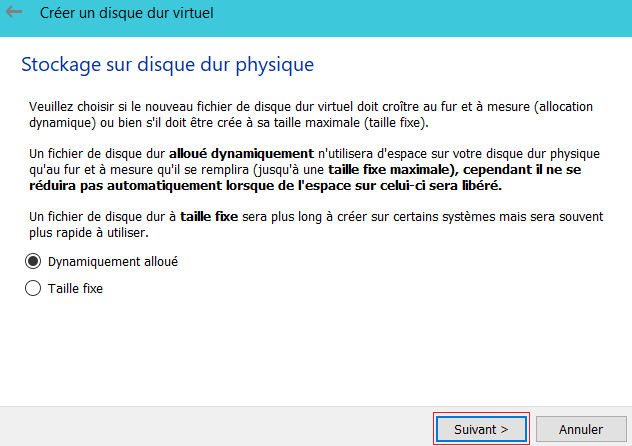
\includegraphics[scale=0.5]{Kerberos/6.png}
         \caption{Ajout de l'utilisateur apache dans l'AD}
         \label{Debian_screenshots/Config/5}
     \end{center}
  \end{figure}
  \FloatBarrier
  
  Entrer la ligne de commande suivante : 
  \begin{minted}{powershell}
  ktpass.exe -princ HTTP/infra01.epitaf.local@EPITAF.LOCAL \ 
  -mapuser apache@EPITAF.LOCAL -pass * \ 
  -crypto AES256-SHA1 -ptype KRB5_NT_PRINCIPAL \ 
  -out C:\http.keytab
  \end{minted}
  
  Lorsque le prompt le demande, entrer le mot de passe, puis entrer la ligne de commande suivante :
   \begin{minted}{powershell}
   ktpass.exe -princ HTTPS/infra01.epitaf.local@EPITAF.LOCAL \ 
        -mapuser apache@EPITAF.LOCAL -pass * \ 
        -crypto AES256-SHA1 -ptype KRB5_NT_PRINCIPAL \ 
        -out C:\https.keytab
  \end{minted}
  
Lorsque le prompt le demande, entrer le mot de passe.

\pagebreak
 Nous venons de créer le service et mapper l'utilisateur apache dessus. La commande nous a généré deux fichiers keytab, essentiels pour qu'Apache2 puisse nous fournir le service attendu.   
  \begin{figure}[h!]
     \begin{center}
         \includegraphics[scale=0.5]{Kerberos/ktpass.png}
         \caption{Schéma de la négociation avec le KDC}
         \label{Debian_screenshots/Config/5}
     \end{center}
  \end{figure}
  \FloatBarrier

\subsection{Configuration du client Kerberos pour un client hors Active Directory}
La version client de kerberos pour Windows et linux se trouve ici : \url{https://web.mit.edu/kerberos/dist/}. \
Sur un debian, il suffit d'installer le paquet \textbf{krb5-user} : 
\begin{minted}{shell}
$ sudo apt install krb5-user
\end{minted}

Il suffit ensuite de : 
\begin{itemize}
    \item Modifier le fichier de configuration 
 \textbf{/etc/krb5.conf} comme présenté dans le fichier template d'ansible
    \item Utiliser \texttt{kinit} pour obtenir un ticket de l'utilisateur voulu
    \item Utiliser \texttt{klist} pour vérifier l'état du cache
    \item Utiliser \texttt{kvno} (optionnel) pour obtenir un TGS du service voulu
     \begin{figure}[h!]
     \begin{center}
         \includegraphics[scale=0.5]{Kerberos/k.png}
         \caption{Obtention des tickets sur une machine linux}
         \label{Debian_screenshots/Config/5}
     \end{center}
  \end{figure}
  \FloatBarrier
  
  \item Pour pouvoir accéder au site hébergé sur INFRA01 via le navigateur web, il faut : 
  \begin{itemize}
      \item Ouvrir \texttt{Firefox} et entrer dans l'url : {\NoAutoSpacing\textbf{about:config}}
        \begin{figure}[h!]
     \begin{center}
         \includegraphics[scale=0.3]{Kerberos/firefox1.png}
         \caption{Configuration de firefox pour kerberos - {\NoAutoSpacing about:config}}
         \label{Debian_screenshots/Config/5}
     \end{center}
  \end{figure}

\pagebreak
  \item Cliquer sur \textbf{J'accepte le risque} et entrer dans la barre de recherche : \textbf{network.negotiate-auth.trusted-uris} ; cliquer ensuite sur \textbf{network.negotiate-auth.trusted-uris}  
     \begin{figure}[h!]
     \begin{center}
         \includegraphics[scale=0.3]{Kerberos/firefox2.png}
         \caption{Configuration de firefox pour kerberos - network}
         \label{Debian_screenshots/Config/5}
     \end{center}
  \end{figure}
  \FloatBarrier
  
  \item Entrer la valeur {\NoAutoSpacing \textbf{192.168.3.2:1000}} et cliquer sur \textit{Ok}.
    \begin{figure}[h!]
     \begin{center}
         \includegraphics[scale=0.3]{Kerberos/firefox3.png}
         \caption{Configuration de firefox pour kerberos - valeur du serveur}
         \label{Debian_screenshots/Config/5}
     \end{center}
  \end{figure}
  \FloatBarrier
  \end{itemize}

\pagebreak
  \item Entrer dans l'url : {\NoAutoSpacing \textbf{192.168.3.2:10000}} et appuyer sur \textit{Entrée}. Le wordpress devrait être accessible.
   \begin{figure}[h!]
     \begin{center}
         \includegraphics[scale=0.3]{Kerberos/firefox4.png}
         \caption{Accès au wordpress après authentification avec kerberos}
         \label{Debian_screenshots/Config/5}
     \end{center}
  \end{figure}
  \FloatBarrier
\end{itemize}

\subsection{Configuration du serveur Apache avec Kerberos}

Pour pouvoir utiliser Kerberos avec apache et respecter les contraintes imposées, il faut : 
\begin{itemize}
    \item Installer libapache2-mod-auth-kerb :
    \begin{minted}{shell}
    $ sudo apt install libapache2-mod-auth-kerb
    \end{minted}
    
    \item Activer le module auth\_kerb :
    \begin{minted}{shell}
    $ sudo a2enmod auth_kerb
    \end{minted}
    
    \item Ajouter dans la configuration apache :
    \begin{minted}{xml}
    <VirtualHost *:10000>
        ServerAdmin wordpress@localhost
        DocumentRoot /var/www/html/wordpress/

        ErrorLog ${APACHE_LOG_DIR}/error.log
        CustomLog ${APACHE_LOG_DIR}/access.log combined
        DirectoryIndex index.php

        SSLEngine on
        SSLCertificateFile "/etc/apache2/server.crt"
        SSLCertificateKeyFile "/etc/apache2/server.key"


        <Directory "/var/www">
                Order deny,allow
                Deny from all
                Allow from 192.168.2.0/24

                AuthType Kerberos
                AuthName "Kerberos Auth"
                KrbAuthRealms EPITAF.LOCAL
                KrbServiceName HTTPS
                Krb5Keytab /etc/apache2/https.keytab
                KrbMethodNegotiate on
                KrbMethodK5Passwd off
                KrbVerifyKDC on
                Require valid-user
        </Directory>

</VirtualHost>
    \end{minted}
    \item Importer les keytabs https.keytab et http.keytab dans \textbf{/etc/apache2/}
    \item Configurer kerberos avec le fichier \textbf{/etc/krb5.conf}. 
    \item Utiliser les commande : 
        \begin{minted}{shell}
    $ sudo chown www-data:root /etc/http*.keytab
    $ sudo chmod 640 /etc/http*.keytab
    \end{minted}
    \item Redémarrer apache :
    \begin{minted}{shell}
    $ sudo systemctl restart apache2
    \end{minted}
\end{itemize}
